\section{System Overview and Problem Formulation}
\subsection{System Architecture}
The proposed system forms a closed-loop perception, geometric modeling and control pipeline, as illustrated in Fig.~\ref{fig:overview}. The input consists of RGB-D images captured above the conveyor. The semantic perception module first segments baggage instances and suppresses tag-like visual interference. The geometric consistency module projects the selected mask into a point cloud, removes residual 3D outliers, and estimates a temporally stable OBB. The dynamic control module then predicts the target state, plans a coarse-to-fine interception trajectory, and executes grasping. If the uncertainty of the target state becomes too high, the active state-regulation module triggers a reset behavior.

\begin{figure*}[!t]
\centering
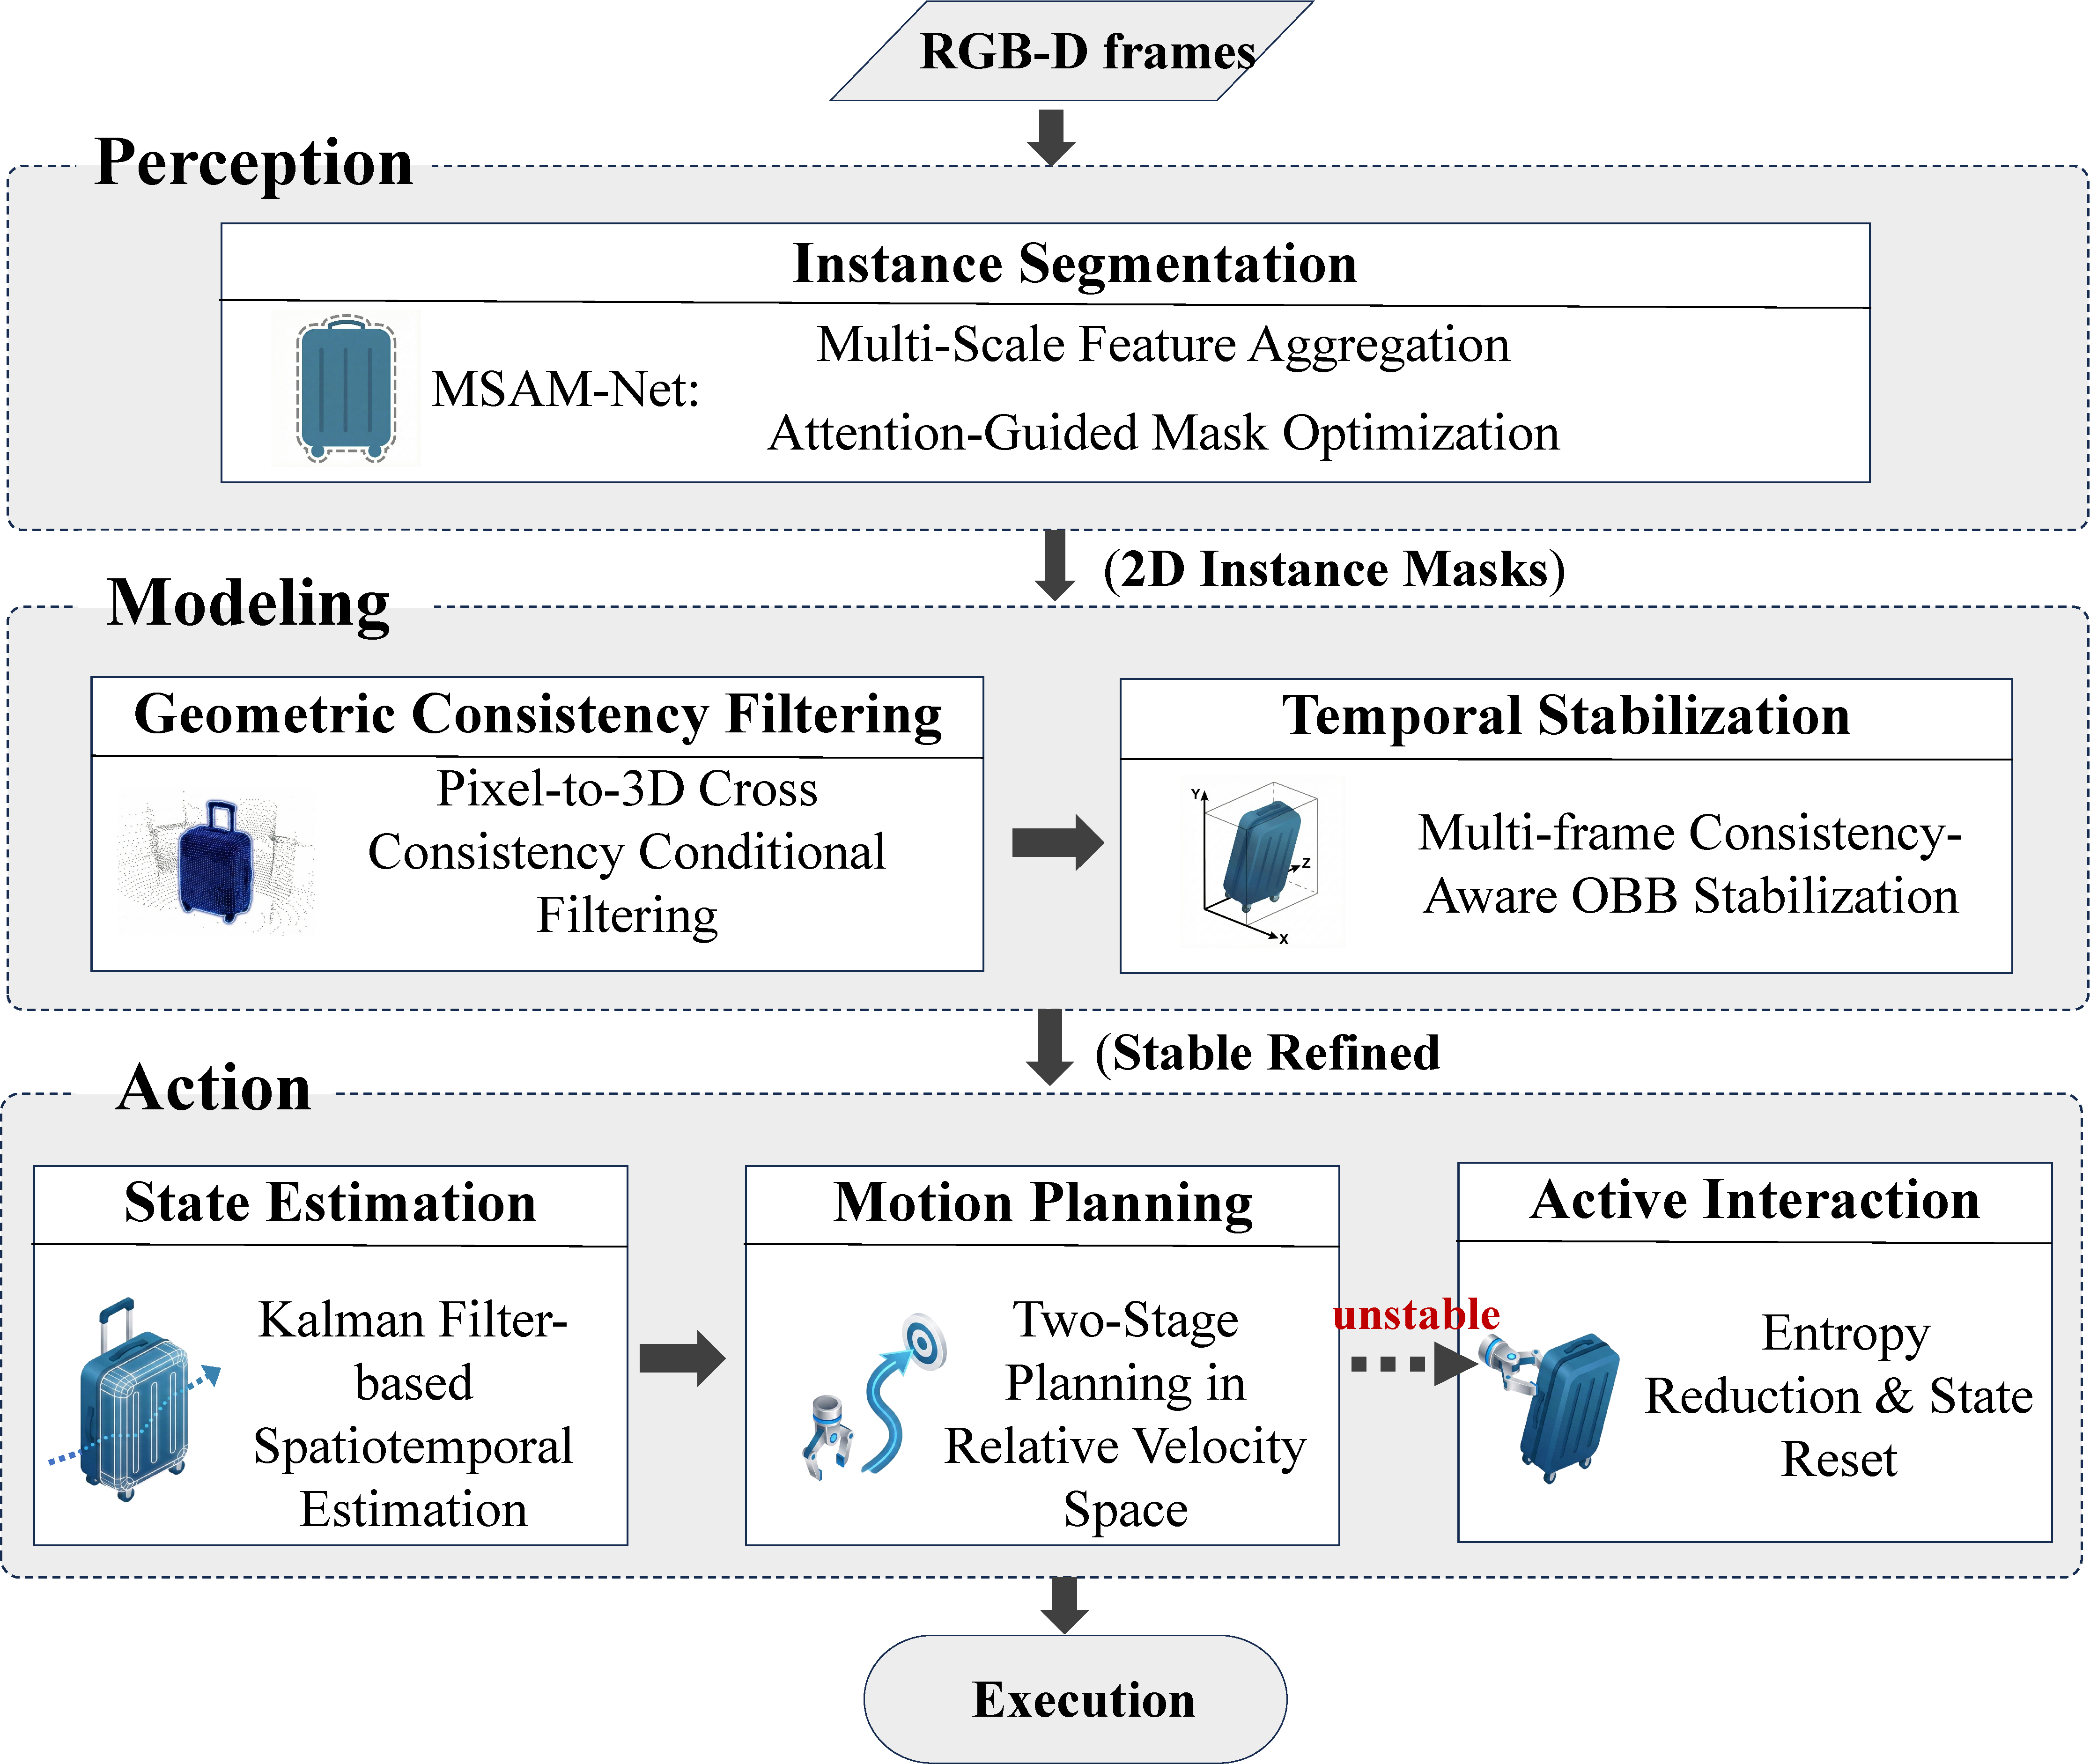
\includegraphics[width=\textwidth]{figures/fig1.pdf}
\caption{Overall framework of the proposed closed-loop perception, geometric modeling, and control system. RGB-D frames are first processed through instance segmentation (MSAM-Net) for mask refinement. The resulting point clouds undergo geometric consistency filtering (PX3C) and temporal stabilization (CAOS) to produce a reliable 3D representation. State estimation uses a Kalman-filter-based spatiotemporal approach, followed by two-stage motion planning in relative velocity space. Active interaction reduces environmental entropy and resets unstable object states, enabling robust real-time execution.}
\label{fig:overview}
\end{figure*}

The central design principle is to avoid irreversible error propagation. A segmentation error can create 3D outliers, a distorted OBB can produce an incorrect grasp pose, and an inaccurate pose can further cause poor placement. Therefore, each stage is designed to evaluate and refine the information passed to the next stage. The framework also closes the loop at the physical level: when passive perception is insufficient, the robot actively changes the state of the baggage to recover observability.

\subsection{Task Definition}
Let $\mathcal{I}_{t}=(I_{t}^{\text{rgb}},I_{t}^{d})$ denote the RGB-D observation at time $t$. The system estimates an object state
\begin{equation}
\boldsymbol{b}_{t}=\{\boldsymbol{p}_{t},\boldsymbol{R}_{t},\boldsymbol{s}_{t}\},
\end{equation}
where $\boldsymbol{p}_{t}$, $\boldsymbol{R}_{t}$, and $\boldsymbol{s}_{t}$ denote the centroid, orientation, and size of the target baggage, respectively. Given the current robot end-effector state $\boldsymbol{x}^{\text{EE}}_{t}$ and the predicted target state $\widehat{\boldsymbol{b}}_{t+\Delta}$, the objective is to generate a grasp trajectory that reaches a feasible suction pose with bounded position and yaw errors. In the experiments, precision success requires a position error below 2$\mathrm{cm}$ and a yaw error below $5^{\circ}$.